\documentclass[1p]{elsarticle_modified}
%\bibliographystyle{elsarticle-num}

%\usepackage[colorlinks]{hyperref}
%\usepackage{abbrmath_seonhwa} %\Abb, \Ascr, \Acal ,\Abf, \Afrak
\usepackage{amsfonts}
\usepackage{amssymb}
\usepackage{amsmath}
\usepackage{amsthm}
\usepackage{scalefnt}
\usepackage{amsbsy}
\usepackage{kotex}
\usepackage{caption}
\usepackage{subfig}
\usepackage{color}
\usepackage{graphicx}
\usepackage{xcolor} %% white, black, red, green, blue, cyan, magenta, yellow
\usepackage{float}
\usepackage{setspace}
\usepackage{hyperref}

\usepackage{tikz}
\usetikzlibrary{arrows}

\usepackage{multirow}
\usepackage{array} % fixed length table
\usepackage{hhline}

%%%%%%%%%%%%%%%%%%%%%
\makeatletter
\renewcommand*\env@matrix[1][\arraystretch]{%
	\edef\arraystretch{#1}%
	\hskip -\arraycolsep
	\let\@ifnextchar\new@ifnextchar
	\array{*\c@MaxMatrixCols c}}
\makeatother %https://tex.stackexchange.com/questions/14071/how-can-i-increase-the-line-spacing-in-a-matrix
%%%%%%%%%%%%%%%

\usepackage[normalem]{ulem}

\newcommand{\msout}[1]{\ifmmode\text{\sout{\ensuremath{#1}}}\else\sout{#1}\fi}
%SOURCE: \msout is \stkout macro in https://tex.stackexchange.com/questions/20609/strikeout-in-math-mode

\newcommand{\cancel}[1]{
	\ifmmode
	{\color{red}\msout{#1}}
	\else
	{\color{red}\sout{#1}}
	\fi
}

\newcommand{\add}[1]{
	{\color{blue}\uwave{#1}}
}

\newcommand{\replace}[2]{
	\ifmmode
	{\color{red}\msout{#1}}{\color{blue}\uwave{#2}}
	\else
	{\color{red}\sout{#1}}{\color{blue}\uwave{#2}}
	\fi
}

\newcommand{\Sol}{\mathcal{S}} %segment
\newcommand{\D}{D} %diagram
\newcommand{\A}{\mathcal{A}} %arc


%%%%%%%%%%%%%%%%%%%%%%%%%%%%%5 test

\def\sl{\operatorname{\textup{SL}}(2,\Cbb)}
\def\psl{\operatorname{\textup{PSL}}(2,\Cbb)}
\def\quan{\mkern 1mu \triangleright \mkern 1mu}

\theoremstyle{definition}
\newtheorem{thm}{Theorem}[section]
\newtheorem{prop}[thm]{Proposition}
\newtheorem{lem}[thm]{Lemma}
\newtheorem{ques}[thm]{Question}
\newtheorem{cor}[thm]{Corollary}
\newtheorem{defn}[thm]{Definition}
\newtheorem{exam}[thm]{Example}
\newtheorem{rmk}[thm]{Remark}
\newtheorem{alg}[thm]{Algorithm}

\newcommand{\I}{\sqrt{-1}}
\begin{document}

%\begin{frontmatter}
%
%\title{Boundary parabolic representations of knots up to 8 crossings}
%
%%% Group authors per affiliation:
%\author{Yunhi Cho} 
%\address{Department of Mathematics, University of Seoul, Seoul, Korea}
%\ead{yhcho@uos.ac.kr}
%
%
%\author{Seonhwa Kim} %\fnref{s_kim}}
%\address{Center for Geometry and Physics, Institute for Basic Science, Pohang, 37673, Korea}
%\ead{ryeona17@ibs.re.kr}
%
%\author{Hyuk Kim}
%\address{Department of Mathematical Sciences, Seoul National University, Seoul 08826, Korea}
%\ead{hyukkim@snu.ac.kr}
%
%\author{Seokbeom Yoon}
%\address{Department of Mathematical Sciences, Seoul National University, Seoul, 08826,  Korea}
%\ead{sbyoon15@snu.ac.kr}
%
%\begin{abstract}
%We find all boundary parabolic representation of knots up to 8 crossings.
%
%\end{abstract}
%\begin{keyword}
%    \MSC[2010] 57M25 
%\end{keyword}
%
%\end{frontmatter}

%\linenumbers
%\tableofcontents
%
\newcommand\colored[1]{\textcolor{white}{\rule[-0.35ex]{0.8em}{1.4ex}}\kern-0.8em\color{red} #1}%
%\newcommand\colored[1]{\textcolor{white}{ #1}\kern-2.17ex	\textcolor{white}{ #1}\kern-1.81ex	\textcolor{white}{ #1}\kern-2.15ex\color{red}#1	}

{\Large $\underline{11a_{106}~(K11a_{106})}$}

\setlength{\tabcolsep}{10pt}
\renewcommand{\arraystretch}{1.6}
\vspace{1cm}\begin{tabular}{m{100pt}>{\centering\arraybackslash}m{274pt}}
\multirow{5}{120pt}{
	\centering
	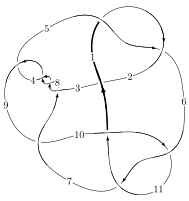
\includegraphics[width=112pt]{../../../GIT/diagram.site/Diagrams/png/355_11a_106.png}\\
\ \ \ A knot diagram\footnotemark}&
\allowdisplaybreaks
\textbf{Linearized knot diagam} \\
\cline{2-2}
 &
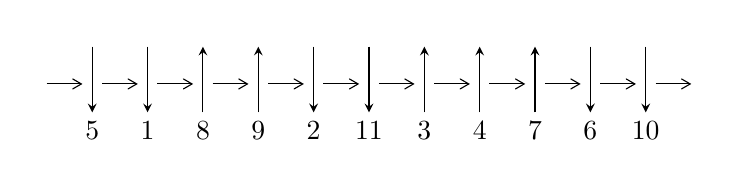
\begin{tikzpicture}[x=20pt, y=17pt]
	% nodes
	\node (C0) at (0, 0) {};
	\node (C1) at (1, 0) {};
	\node (C1U) at (1, +1) {};
	\node (C1D) at (1, -1) {5};

	\node (C2) at (2, 0) {};
	\node (C2U) at (2, +1) {};
	\node (C2D) at (2, -1) {1};

	\node (C3) at (3, 0) {};
	\node (C3U) at (3, +1) {};
	\node (C3D) at (3, -1) {8};

	\node (C4) at (4, 0) {};
	\node (C4U) at (4, +1) {};
	\node (C4D) at (4, -1) {9};

	\node (C5) at (5, 0) {};
	\node (C5U) at (5, +1) {};
	\node (C5D) at (5, -1) {2};

	\node (C6) at (6, 0) {};
	\node (C6U) at (6, +1) {};
	\node (C6D) at (6, -1) {11};

	\node (C7) at (7, 0) {};
	\node (C7U) at (7, +1) {};
	\node (C7D) at (7, -1) {3};

	\node (C8) at (8, 0) {};
	\node (C8U) at (8, +1) {};
	\node (C8D) at (8, -1) {4};

	\node (C9) at (9, 0) {};
	\node (C9U) at (9, +1) {};
	\node (C9D) at (9, -1) {7};

	\node (C10) at (10, 0) {};
	\node (C10U) at (10, +1) {};
	\node (C10D) at (10, -1) {6};

	\node (C11) at (11, 0) {};
	\node (C11U) at (11, +1) {};
	\node (C11D) at (11, -1) {10};
	\node (C12) at (12, 0) {};

	% arrows
	\draw[->,>={angle 60}]
	(C0) edge (C1) (C1) edge (C2) (C2) edge (C3) (C3) edge (C4) (C4) edge (C5) (C5) edge (C6) (C6) edge (C7) (C7) edge (C8) (C8) edge (C9) (C9) edge (C10) (C10) edge (C11) (C11) edge (C12) ;	\draw[->,>=stealth]
	(C1U) edge (C1D) (C2U) edge (C2D) (C3D) edge (C3U) (C4D) edge (C4U) (C5U) edge (C5D) (C6U) edge (C6D) (C7D) edge (C7U) (C8D) edge (C8U) (C9D) edge (C9U) (C10U) edge (C10D) (C11U) edge (C11D) ;
	\end{tikzpicture} \\
\hhline{~~} \\& 
\textbf{Solving Sequence} \\ \cline{2-2} 
 &
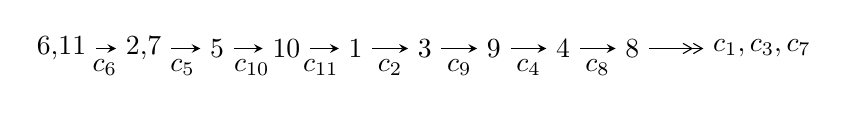
\begin{tikzpicture}[x=25pt, y=7pt]
	% node
	\node (A0) at (-1/8, 0) {6,11};
	\node (A1) at (17/16, 0) {2,7};
	\node (A2) at (17/8, 0) {5};
	\node (A3) at (25/8, 0) {10};
	\node (A4) at (33/8, 0) {1};
	\node (A5) at (41/8, 0) {3};
	\node (A6) at (49/8, 0) {9};
	\node (A7) at (57/8, 0) {4};
	\node (A8) at (65/8, 0) {8};
	\node (C1) at (1/2, -1) {$c_{6}$};
	\node (C2) at (13/8, -1) {$c_{5}$};
	\node (C3) at (21/8, -1) {$c_{10}$};
	\node (C4) at (29/8, -1) {$c_{11}$};
	\node (C5) at (37/8, -1) {$c_{2}$};
	\node (C6) at (45/8, -1) {$c_{9}$};
	\node (C7) at (53/8, -1) {$c_{4}$};
	\node (C8) at (61/8, -1) {$c_{8}$};
	\node (A9) at (10, 0) {$c_{1},c_{3},c_{7}$};

	% edge
	\draw[->,>=stealth]	
	(A0) edge (A1) (A1) edge (A2) (A2) edge (A3) (A3) edge (A4) (A4) edge (A5) (A5) edge (A6) (A6) edge (A7) (A7) edge (A8) ;
	\draw[->>,>={angle 60}]	
	(A8) edge (A9);
\end{tikzpicture} \\ 

\end{tabular} \\

\footnotetext{
The image of knot diagram is generated by the software ``\textbf{Draw programme}" developed by Andrew Bartholomew(\url{http://www.layer8.co.uk/maths/draw/index.htm\#Running-draw}), where we modified some parts for our purpose(\url{https://github.com/CATsTAILs/LinksPainter}).
}\phantom \\ \newline 
\centering \textbf{Ideals for irreducible components\footnotemark of $X_{\text{par}}$} 
 
\begin{align*}
I^u_{1}&=\langle 
b- u,\\
\phantom{I^u_{1}}&\phantom{= \langle  }u^{17}- u^{16}-3 u^{15}+4 u^{14}+6 u^{13}-9 u^{12}-4 u^{11}+11 u^{10}+2 u^9-9 u^8+4 u^7+4 u^6-2 u^4+4 u^3+u^2+2 a+2 u-1,\\
\phantom{I^u_{1}}&\phantom{= \langle  }u^{19}- u^{18}+\cdots-2 u^2+1\rangle \\
I^u_{2}&=\langle 
-37263 u^{29}-111490 u^{28}+\cdots+162577 b+113039,\\
\phantom{I^u_{2}}&\phantom{= \langle  }125314 u^{29}-274067 u^{28}+\cdots+162577 a+438193,\;u^{30}- u^{29}+\cdots+2 u-1\rangle \\
I^u_{3}&=\langle 
b+1,\;a+2,\;u-1\rangle \\
I^u_{4}&=\langle 
b-1,\;a^2-4 a+2,\;u+1\rangle \\
\\
\end{align*}
\raggedright * 4 irreducible components of $\dim_{\mathbb{C}}=0$, with total 52 representations.\\
\footnotetext{All coefficients of polynomials are rational numbers. But the coefficients are sometimes approximated in decimal forms when there is not enough margin.}
\newpage
\renewcommand{\arraystretch}{1}
\centering \section*{I. $I^u_{1}= \langle b- u,\;u^{17}- u^{16}+\cdots+2 a-1,\;u^{19}- u^{18}+\cdots-2 u^2+1 \rangle$}
\flushleft \textbf{(i) Arc colorings}\\
\begin{tabular}{m{7pt} m{180pt} m{7pt} m{180pt} }
\flushright $a_{6}=$&$\begin{pmatrix}1\\0\end{pmatrix}$ \\
\flushright $a_{11}=$&$\begin{pmatrix}0\\u\end{pmatrix}$ \\
\flushright $a_{2}=$&$\begin{pmatrix}-\frac{1}{2} u^{17}+\frac{1}{2} u^{16}+\cdots- u+\frac{1}{2}\\u\end{pmatrix}$ \\
\flushright $a_{7}=$&$\begin{pmatrix}1\\u^2\end{pmatrix}$ \\
\flushright $a_{5}=$&$\begin{pmatrix}\frac{1}{2} u^{18}-\frac{1}{2} u^{17}+\cdots-\frac{1}{2} u+1\\- u^2\end{pmatrix}$ \\
\flushright $a_{10}=$&$\begin{pmatrix}u\\u\end{pmatrix}$ \\
\flushright $a_{1}=$&$\begin{pmatrix}- u^3\\- u^3+u\end{pmatrix}$ \\
\flushright $a_{3}=$&$\begin{pmatrix}-\frac{1}{2} u^{17}+\frac{1}{2} u^{16}+\cdots- u+\frac{1}{2}\\u^5- u^3+u\end{pmatrix}$ \\
\flushright $a_{9}=$&$\begin{pmatrix}u^3\\u^5- u^3+u\end{pmatrix}$ \\
\flushright $a_{4}=$&$\begin{pmatrix}u^{18}- u^{17}+\cdots- u+1\\\frac{1}{2} u^{18}-\frac{1}{2} u^{17}+\cdots+\frac{1}{2} u^3-\frac{1}{2} u\end{pmatrix}$ \\
\flushright $a_{8}=$&$\begin{pmatrix}u^{18}-\frac{3}{2} u^{17}+\cdots-2 u+\frac{3}{2}\\-\frac{1}{2} u^{18}+\frac{1}{2} u^{17}+\cdots-\frac{1}{2} u^3+\frac{1}{2} u\end{pmatrix}$\\ \flushright $a_{8}=$&$\begin{pmatrix}u^{18}-\frac{3}{2} u^{17}+\cdots-2 u+\frac{3}{2}\\-\frac{1}{2} u^{18}+\frac{1}{2} u^{17}+\cdots-\frac{1}{2} u^3+\frac{1}{2} u\end{pmatrix}$\\&\end{tabular}
\flushleft \textbf{(ii) Obstruction class $= -1$}\\~\\
\flushleft \textbf{(iii) Cusp Shapes $= 2 u^{18}- u^{17}-9 u^{16}+5 u^{15}+26 u^{14}-14 u^{13}-43 u^{12}+26 u^{11}+51 u^{10}-34 u^9-31 u^8+32 u^7+12 u^6-20 u^5+6 u^4+10 u^3+5 u^2-4 u-1$}\\~\\
\newpage\renewcommand{\arraystretch}{1}
\flushleft \textbf{(iv) u-Polynomials at the component}\newline \\
\begin{tabular}{m{50pt}|m{274pt}}
Crossings & \hspace{64pt}u-Polynomials at each crossing \\
\hline $$\begin{aligned}c_{1},c_{5},c_{6}\\c_{10}\end{aligned}$$&$\begin{aligned}
&u^{19}+u^{18}+\cdots+2 u^2-1
\end{aligned}$\\
\hline $$\begin{aligned}c_{2},c_{11}\end{aligned}$$&$\begin{aligned}
&u^{19}+9 u^{18}+\cdots+4 u+1
\end{aligned}$\\
\hline $$\begin{aligned}c_{3},c_{4},c_{7}\\c_{8}\end{aligned}$$&$\begin{aligned}
&u^{19}+3 u^{18}+\cdots+2 u-2
\end{aligned}$\\
\hline $$\begin{aligned}c_{9}\end{aligned}$$&$\begin{aligned}
&u^{19}+3 u^{18}+\cdots+16 u-16
\end{aligned}$\\
\hline
\end{tabular}\\~\\
\newpage\renewcommand{\arraystretch}{1}
\flushleft \textbf{(v) Riley Polynomials at the component}\newline \\
\begin{tabular}{m{50pt}|m{274pt}}
Crossings & \hspace{64pt}Riley Polynomials at each crossing \\
\hline $$\begin{aligned}c_{1},c_{5},c_{6}\\c_{10}\end{aligned}$$&$\begin{aligned}
&y^{19}-9 y^{18}+\cdots+4 y-1
\end{aligned}$\\
\hline $$\begin{aligned}c_{2},c_{11}\end{aligned}$$&$\begin{aligned}
&y^{19}+7 y^{18}+\cdots-4 y-1
\end{aligned}$\\
\hline $$\begin{aligned}c_{3},c_{4},c_{7}\\c_{8}\end{aligned}$$&$\begin{aligned}
&y^{19}-21 y^{18}+\cdots-4 y-4
\end{aligned}$\\
\hline $$\begin{aligned}c_{9}\end{aligned}$$&$\begin{aligned}
&y^{19}+7 y^{18}+\cdots+2816 y-256
\end{aligned}$\\
\hline
\end{tabular}\\~\\
\newpage\flushleft \textbf{(vi) Complex Volumes and Cusp Shapes}
$$\begin{array}{c|c|c}  
\text{Solutions to }I^u_{1}& \I (\text{vol} + \sqrt{-1}CS) & \text{Cusp shape}\\
 \hline 
\begin{aligned}
u &= -0.812789 + 0.553417 I \\
a &= -0.76890 - 1.22204 I \\
b &= -0.812789 + 0.553417 I\end{aligned}
 & \phantom{-}1.82665 + 4.33190 I & \phantom{-}3.09756 - 7.93622 I \\ \hline\begin{aligned}
u &= -0.812789 - 0.553417 I \\
a &= -0.76890 + 1.22204 I \\
b &= -0.812789 - 0.553417 I\end{aligned}
 & \phantom{-}1.82665 - 4.33190 I & \phantom{-}3.09756 + 7.93622 I \\ \hline\begin{aligned}
u &= \phantom{-}0.865007 + 0.704905 I \\
a &= \phantom{-}1.072110 - 0.840866 I \\
b &= \phantom{-}0.865007 + 0.704905 I\end{aligned}
 & \phantom{-}10.08310 - 5.40272 I & \phantom{-}4.82648 + 5.68964 I \\ \hline\begin{aligned}
u &= \phantom{-}0.865007 - 0.704905 I \\
a &= \phantom{-}1.072110 + 0.840866 I \\
b &= \phantom{-}0.865007 - 0.704905 I\end{aligned}
 & \phantom{-}10.08310 + 5.40272 I & \phantom{-}4.82648 - 5.68964 I \\ \hline\begin{aligned}
u &= \phantom{-}0.347731 + 0.806765 I \\
a &= \phantom{-}0.287964 - 0.269780 I \\
b &= \phantom{-}0.347731 + 0.806765 I\end{aligned}
 & \phantom{-}8.56139 + 2.84598 I & \phantom{-}6.12727 - 0.57057 I \\ \hline\begin{aligned}
u &= \phantom{-}0.347731 - 0.806765 I \\
a &= \phantom{-}0.287964 + 0.269780 I \\
b &= \phantom{-}0.347731 - 0.806765 I\end{aligned}
 & \phantom{-}8.56139 - 2.84598 I & \phantom{-}6.12727 + 0.57057 I \\ \hline\begin{aligned}
u &= -1.072710 + 0.432309 I \\
a &= -1.91340 - 1.91365 I \\
b &= -1.072710 + 0.432309 I\end{aligned}
 & \phantom{-}0.89681 + 2.96240 I & -1.25513 - 4.67576 I \\ \hline\begin{aligned}
u &= -1.072710 - 0.432309 I \\
a &= -1.91340 + 1.91365 I \\
b &= -1.072710 - 0.432309 I\end{aligned}
 & \phantom{-}0.89681 - 2.96240 I & -1.25513 + 4.67576 I \\ \hline\begin{aligned}
u &= \phantom{-}1.135950 + 0.496880 I \\
a &= \phantom{-}2.09240 - 1.47882 I \\
b &= \phantom{-}1.135950 + 0.496880 I\end{aligned}
 & -4.68926 - 6.06103 I & -4.96256 + 4.06889 I \\ \hline\begin{aligned}
u &= \phantom{-}1.135950 - 0.496880 I \\
a &= \phantom{-}2.09240 + 1.47882 I \\
b &= \phantom{-}1.135950 - 0.496880 I\end{aligned}
 & -4.68926 + 6.06103 I & -4.96256 - 4.06889 I\\
 \hline 
 \end{array}$$\newpage$$\begin{array}{c|c|c}  
\text{Solutions to }I^u_{1}& \I (\text{vol} + \sqrt{-1}CS) & \text{Cusp shape}\\
 \hline 
\begin{aligned}
u &= \phantom{-}0.651125 + 0.371544 I \\
a &= -0.115490 - 1.188520 I \\
b &= \phantom{-}0.651125 + 0.371544 I\end{aligned}
 & -0.69486 - 1.46005 I & -2.24162 + 4.71190 I \\ \hline\begin{aligned}
u &= \phantom{-}0.651125 - 0.371544 I \\
a &= -0.115490 + 1.188520 I \\
b &= \phantom{-}0.651125 - 0.371544 I\end{aligned}
 & -0.69486 + 1.46005 I & -2.24162 - 4.71190 I \\ \hline\begin{aligned}
u &= -1.171910 + 0.539955 I \\
a &= -2.14090 - 1.24940 I \\
b &= -1.171910 + 0.539955 I\end{aligned}
 & -3.93034 + 10.41950 I & -3.27524 - 9.24443 I \\ \hline\begin{aligned}
u &= -1.171910 - 0.539955 I \\
a &= -2.14090 + 1.24940 I \\
b &= -1.171910 - 0.539955 I\end{aligned}
 & -3.93034 - 10.41950 I & -3.27524 + 9.24443 I \\ \hline\begin{aligned}
u &= -0.686077\phantom{ +0.000000I} \\
a &= \phantom{-}1.90633\phantom{ +0.000000I} \\
b &= -0.686077\phantom{ +0.000000I}\end{aligned}
 & \phantom{-}2.96406\phantom{ +0.000000I} & \phantom{-}4.32400\phantom{ +0.000000I} \\ \hline\begin{aligned}
u &= -0.296841 + 0.610442 I \\
a &= -0.117122 - 0.390719 I \\
b &= -0.296841 + 0.610442 I\end{aligned}
 & \phantom{-}1.19212 - 1.04367 I & \phantom{-}4.57560 + 2.19936 I \\ \hline\begin{aligned}
u &= -0.296841 - 0.610442 I \\
a &= -0.117122 + 0.390719 I \\
b &= -0.296841 - 0.610442 I\end{aligned}
 & \phantom{-}1.19212 + 1.04367 I & \phantom{-}4.57560 - 2.19936 I \\ \hline\begin{aligned}
u &= \phantom{-}1.197470 + 0.579281 I \\
a &= \phantom{-}2.15018 - 1.07944 I \\
b &= \phantom{-}1.197470 + 0.579281 I\end{aligned}
 & \phantom{-}3.36659 - 13.40010 I & -0.05434 + 8.12876 I \\ \hline\begin{aligned}
u &= \phantom{-}1.197470 - 0.579281 I \\
a &= \phantom{-}2.15018 + 1.07944 I \\
b &= \phantom{-}1.197470 - 0.579281 I\end{aligned}
 & \phantom{-}3.36659 + 13.40010 I & -0.05434 - 8.12876 I\\
 \hline 
 \end{array}$$\newpage\newpage\renewcommand{\arraystretch}{1}
\centering \section*{II. $I^u_{2}= \langle -3.73\times10^{4} u^{29}-1.11\times10^{5} u^{28}+\cdots+1.63\times10^{5} b+1.13\times10^{5},\;1.25\times10^{5} u^{29}-2.74\times10^{5} u^{28}+\cdots+1.63\times10^{5} a+4.38\times10^{5},\;u^{30}- u^{29}+\cdots+2 u-1 \rangle$}
\flushleft \textbf{(i) Arc colorings}\\
\begin{tabular}{m{7pt} m{180pt} m{7pt} m{180pt} }
\flushright $a_{6}=$&$\begin{pmatrix}1\\0\end{pmatrix}$ \\
\flushright $a_{11}=$&$\begin{pmatrix}0\\u\end{pmatrix}$ \\
\flushright $a_{2}=$&$\begin{pmatrix}-0.770798 u^{29}+1.68577 u^{28}+\cdots+0.897808 u-2.69530\\0.229202 u^{29}+0.685767 u^{28}+\cdots-1.10219 u-0.695295\end{pmatrix}$ \\
\flushright $a_{7}=$&$\begin{pmatrix}1\\u^2\end{pmatrix}$ \\
\flushright $a_{5}=$&$\begin{pmatrix}0.219674 u^{29}+0.569613 u^{28}+\cdots+3.03192 u-2.26358\\0.914970 u^{29}-0.354884 u^{28}+\cdots-1.15370 u-0.770798\end{pmatrix}$ \\
\flushright $a_{10}=$&$\begin{pmatrix}u\\u\end{pmatrix}$ \\
\flushright $a_{1}=$&$\begin{pmatrix}- u^3\\- u^3+u\end{pmatrix}$ \\
\flushright $a_{3}=$&$\begin{pmatrix}-0.667228 u^{29}+1.85414 u^{28}+\cdots+1.11916 u-3.08601\\0.892857 u^{29}+0.684771 u^{28}+\cdots-3.48157 u-0.171045\end{pmatrix}$ \\
\flushright $a_{9}=$&$\begin{pmatrix}u^3\\u^5- u^3+u\end{pmatrix}$ \\
\flushright $a_{4}=$&$\begin{pmatrix}0.120681 u^{29}+0.253677 u^{28}+\cdots+3.97856 u-2.66124\\1.47694 u^{29}-0.641395 u^{28}+\cdots-1.62083 u-1.34137\end{pmatrix}$ \\
\flushright $a_{8}=$&$\begin{pmatrix}-1.35965 u^{29}+0.714234 u^{28}+\cdots+4.37797 u-3.99301\\0.147635 u^{29}-0.397719 u^{28}+\cdots-1.70941 u-2.11106\end{pmatrix}$\\ \flushright $a_{8}=$&$\begin{pmatrix}-1.35965 u^{29}+0.714234 u^{28}+\cdots+4.37797 u-3.99301\\0.147635 u^{29}-0.397719 u^{28}+\cdots-1.70941 u-2.11106\end{pmatrix}$\\&\end{tabular}
\flushleft \textbf{(ii) Obstruction class $= -1$}\\~\\
\flushleft \textbf{(iii) Cusp Shapes $= -\frac{174400}{162577} u^{29}+\frac{211456}{162577} u^{28}+\cdots-\frac{402552}{162577} u+\frac{413650}{162577}$}\\~\\
\newpage\renewcommand{\arraystretch}{1}
\flushleft \textbf{(iv) u-Polynomials at the component}\newline \\
\begin{tabular}{m{50pt}|m{274pt}}
Crossings & \hspace{64pt}u-Polynomials at each crossing \\
\hline $$\begin{aligned}c_{1},c_{5},c_{6}\\c_{10}\end{aligned}$$&$\begin{aligned}
&u^{30}+u^{29}+\cdots-2 u-1
\end{aligned}$\\
\hline $$\begin{aligned}c_{2},c_{11}\end{aligned}$$&$\begin{aligned}
&u^{30}+17 u^{29}+\cdots+8 u^2+1
\end{aligned}$\\
\hline $$\begin{aligned}c_{3},c_{4},c_{7}\\c_{8}\end{aligned}$$&$\begin{aligned}
&(u^{15}- u^{14}+\cdots-2 u-1)^{2}
\end{aligned}$\\
\hline $$\begin{aligned}c_{9}\end{aligned}$$&$\begin{aligned}
&(u^{15}+3 u^{14}+\cdots-4 u^2+1)^{2}
\end{aligned}$\\
\hline
\end{tabular}\\~\\
\newpage\renewcommand{\arraystretch}{1}
\flushleft \textbf{(v) Riley Polynomials at the component}\newline \\
\begin{tabular}{m{50pt}|m{274pt}}
Crossings & \hspace{64pt}Riley Polynomials at each crossing \\
\hline $$\begin{aligned}c_{1},c_{5},c_{6}\\c_{10}\end{aligned}$$&$\begin{aligned}
&y^{30}-17 y^{29}+\cdots+8 y^2+1
\end{aligned}$\\
\hline $$\begin{aligned}c_{2},c_{11}\end{aligned}$$&$\begin{aligned}
&y^{30}-9 y^{29}+\cdots+16 y+1
\end{aligned}$\\
\hline $$\begin{aligned}c_{3},c_{4},c_{7}\\c_{8}\end{aligned}$$&$\begin{aligned}
&(y^{15}-17 y^{14}+\cdots+8 y-1)^{2}
\end{aligned}$\\
\hline $$\begin{aligned}c_{9}\end{aligned}$$&$\begin{aligned}
&(y^{15}+7 y^{14}+\cdots+8 y-1)^{2}
\end{aligned}$\\
\hline
\end{tabular}\\~\\
\newpage\flushleft \textbf{(vi) Complex Volumes and Cusp Shapes}
$$\begin{array}{c|c|c}  
\text{Solutions to }I^u_{2}& \I (\text{vol} + \sqrt{-1}CS) & \text{Cusp shape}\\
 \hline 
\begin{aligned}
u &= \phantom{-}0.716927 + 0.736174 I \\
a &= \phantom{-}0.0379780 - 0.0389976 I \\
b &= \phantom{-}0.716927 - 0.736174 I\end{aligned}
 & \phantom{-}10.5121\phantom{ +0.000000I} & \phantom{-}5.97706 + 0. I\phantom{ +0.000000I} \\ \hline\begin{aligned}
u &= \phantom{-}0.716927 - 0.736174 I \\
a &= \phantom{-}0.0379780 + 0.0389976 I \\
b &= \phantom{-}0.716927 + 0.736174 I\end{aligned}
 & \phantom{-}10.5121\phantom{ +0.000000I} & \phantom{-}5.97706 + 0. I\phantom{ +0.000000I} \\ \hline\begin{aligned}
u &= \phantom{-}0.246680 + 0.896428 I \\
a &= \phantom{-}0.846092 + 0.456626 I \\
b &= \phantom{-}1.131460 - 0.580385 I\end{aligned}
 & \phantom{-}6.22908 + 8.01682 I & \phantom{-}3.04132 - 4.89679 I \\ \hline\begin{aligned}
u &= \phantom{-}0.246680 - 0.896428 I \\
a &= \phantom{-}0.846092 - 0.456626 I \\
b &= \phantom{-}1.131460 + 0.580385 I\end{aligned}
 & \phantom{-}6.22908 - 8.01682 I & \phantom{-}3.04132 + 4.89679 I \\ \hline\begin{aligned}
u &= \phantom{-}1.12548\phantom{ +0.000000I} \\
a &= -1.67481\phantom{ +0.000000I} \\
b &= -0.786295\phantom{ +0.000000I}\end{aligned}
 & -2.69194\phantom{ +0.000000I} & \phantom{-}4.62820\phantom{ +0.000000I} \\ \hline\begin{aligned}
u &= \phantom{-}1.053770 + 0.396631 I \\
a &= -0.660279 - 0.334663 I \\
b &= \phantom{-}0.170936 - 0.647526 I\end{aligned}
 & -1.99092 - 1.64925 I & -2.39367 + 0.16522 I \\ \hline\begin{aligned}
u &= \phantom{-}1.053770 - 0.396631 I \\
a &= -0.660279 + 0.334663 I \\
b &= \phantom{-}0.170936 + 0.647526 I\end{aligned}
 & -1.99092 + 1.64925 I & -2.39367 - 0.16522 I \\ \hline\begin{aligned}
u &= -0.651659 + 0.523428 I \\
a &= \phantom{-}0.281100 + 0.225787 I \\
b &= -0.651659 - 0.523428 I\end{aligned}
 & \phantom{-}2.23561\phantom{ +0.000000I} & \phantom{-}5.03935 + 0. I\phantom{ +0.000000I} \\ \hline\begin{aligned}
u &= -0.651659 - 0.523428 I \\
a &= \phantom{-}0.281100 - 0.225787 I \\
b &= -0.651659 + 0.523428 I\end{aligned}
 & \phantom{-}2.23561\phantom{ +0.000000I} & \phantom{-}5.03935 + 0. I\phantom{ +0.000000I} \\ \hline\begin{aligned}
u &= -0.212223 + 0.801752 I \\
a &= -0.793447 + 0.659092 I \\
b &= -1.101980 - 0.506508 I\end{aligned}
 & -1.10658 - 5.45324 I & -0.00468 + 6.35130 I\\
 \hline 
 \end{array}$$\newpage$$\begin{array}{c|c|c}  
\text{Solutions to }I^u_{2}& \I (\text{vol} + \sqrt{-1}CS) & \text{Cusp shape}\\
 \hline 
\begin{aligned}
u &= -0.212223 - 0.801752 I \\
a &= -0.793447 - 0.659092 I \\
b &= -1.101980 + 0.506508 I\end{aligned}
 & -1.10658 + 5.45324 I & -0.00468 - 6.35130 I \\ \hline\begin{aligned}
u &= -1.176320 + 0.122445 I \\
a &= \phantom{-}1.120030 - 0.323137 I \\
b &= \phantom{-}0.279034 - 0.410677 I\end{aligned}
 & \phantom{-}3.47397 - 0.15908 I & \phantom{-}1.79403 - 0.85194 I \\ \hline\begin{aligned}
u &= -1.176320 - 0.122445 I \\
a &= \phantom{-}1.120030 + 0.323137 I \\
b &= \phantom{-}0.279034 + 0.410677 I\end{aligned}
 & \phantom{-}3.47397 + 0.15908 I & \phantom{-}1.79403 + 0.85194 I \\ \hline\begin{aligned}
u &= \phantom{-}1.087970 + 0.476458 I \\
a &= -2.06013 + 0.62143 I \\
b &= -1.288900 + 0.283680 I\end{aligned}
 & \phantom{-}1.23287 - 4.11725 I & -1.40312 + 3.71929 I \\ \hline\begin{aligned}
u &= \phantom{-}1.087970 - 0.476458 I \\
a &= -2.06013 - 0.62143 I \\
b &= -1.288900 - 0.283680 I\end{aligned}
 & \phantom{-}1.23287 + 4.11725 I & -1.40312 - 3.71929 I \\ \hline\begin{aligned}
u &= -1.134360 + 0.387877 I \\
a &= \phantom{-}1.99836 + 0.59003 I \\
b &= \phantom{-}1.209080 + 0.320151 I\end{aligned}
 & -5.46412 + 1.81248 I & -5.85619 - 4.33913 I \\ \hline\begin{aligned}
u &= -1.134360 - 0.387877 I \\
a &= \phantom{-}1.99836 - 0.59003 I \\
b &= \phantom{-}1.209080 - 0.320151 I\end{aligned}
 & -5.46412 - 1.81248 I & -5.85619 + 4.33913 I \\ \hline\begin{aligned}
u &= -1.101980 + 0.506508 I \\
a &= \phantom{-}0.536960 - 0.457402 I \\
b &= -0.212223 - 0.801752 I\end{aligned}
 & -1.10658 + 5.45324 I & -0.00468 - 6.35130 I \\ \hline\begin{aligned}
u &= -1.101980 - 0.506508 I \\
a &= \phantom{-}0.536960 + 0.457402 I \\
b &= -0.212223 + 0.801752 I\end{aligned}
 & -1.10658 - 5.45324 I & -0.00468 + 6.35130 I \\ \hline\begin{aligned}
u &= -0.786295\phantom{ +0.000000I} \\
a &= \phantom{-}2.39726\phantom{ +0.000000I} \\
b &= \phantom{-}1.12548\phantom{ +0.000000I}\end{aligned}
 & -2.69194\phantom{ +0.000000I} & \phantom{-}4.62820\phantom{ +0.000000I}\\
 \hline 
 \end{array}$$\newpage$$\begin{array}{c|c|c}  
\text{Solutions to }I^u_{2}& \I (\text{vol} + \sqrt{-1}CS) & \text{Cusp shape}\\
 \hline 
\begin{aligned}
u &= \phantom{-}1.209080 + 0.320151 I \\
a &= -1.90725 + 0.59253 I \\
b &= -1.134360 + 0.387877 I\end{aligned}
 & -5.46412 + 1.81248 I & -5.85619 - 4.33913 I \\ \hline\begin{aligned}
u &= \phantom{-}1.209080 - 0.320151 I \\
a &= -1.90725 - 0.59253 I \\
b &= -1.134360 - 0.387877 I\end{aligned}
 & -5.46412 - 1.81248 I & -5.85619 + 4.33913 I \\ \hline\begin{aligned}
u &= \phantom{-}1.131460 + 0.580385 I \\
a &= -0.453027 - 0.537511 I \\
b &= \phantom{-}0.246680 - 0.896428 I\end{aligned}
 & \phantom{-}6.22908 - 8.01682 I & \phantom{-}3.04132 + 4.89679 I \\ \hline\begin{aligned}
u &= \phantom{-}1.131460 - 0.580385 I \\
a &= -0.453027 + 0.537511 I \\
b &= \phantom{-}0.246680 + 0.896428 I\end{aligned}
 & \phantom{-}6.22908 + 8.01682 I & \phantom{-}3.04132 - 4.89679 I \\ \hline\begin{aligned}
u &= -1.288900 + 0.283680 I \\
a &= \phantom{-}1.82798 + 0.63933 I \\
b &= \phantom{-}1.087970 + 0.476458 I\end{aligned}
 & \phantom{-}1.23287 - 4.11725 I & -1.40312 + 3.71929 I \\ \hline\begin{aligned}
u &= -1.288900 - 0.283680 I \\
a &= \phantom{-}1.82798 - 0.63933 I \\
b &= \phantom{-}1.087970 - 0.476458 I\end{aligned}
 & \phantom{-}1.23287 + 4.11725 I & -1.40312 - 3.71929 I \\ \hline\begin{aligned}
u &= \phantom{-}0.170936 + 0.647526 I \\
a &= \phantom{-}0.672650 + 1.047100 I \\
b &= \phantom{-}1.053770 - 0.396631 I\end{aligned}
 & -1.99092 + 1.64925 I & -2.39367 - 0.16522 I \\ \hline\begin{aligned}
u &= \phantom{-}0.170936 - 0.647526 I \\
a &= \phantom{-}0.672650 - 1.047100 I \\
b &= \phantom{-}1.053770 + 0.396631 I\end{aligned}
 & -1.99092 - 1.64925 I & -2.39367 + 0.16522 I \\ \hline\begin{aligned}
u &= \phantom{-}0.279034 + 0.410677 I \\
a &= -2.30824 + 1.54348 I \\
b &= -1.176320 - 0.122445 I\end{aligned}
 & \phantom{-}3.47397 + 0.15908 I & \phantom{-}1.79403 + 0.85194 I \\ \hline\begin{aligned}
u &= \phantom{-}0.279034 - 0.410677 I \\
a &= -2.30824 - 1.54348 I \\
b &= -1.176320 + 0.122445 I\end{aligned}
 & \phantom{-}3.47397 - 0.15908 I & \phantom{-}1.79403 - 0.85194 I\\
 \hline 
 \end{array}$$\newpage\newpage\renewcommand{\arraystretch}{1}
\centering \section*{III. $I^u_{3}= \langle b+1,\;a+2,\;u-1 \rangle$}
\flushleft \textbf{(i) Arc colorings}\\
\begin{tabular}{m{7pt} m{180pt} m{7pt} m{180pt} }
\flushright $a_{6}=$&$\begin{pmatrix}1\\0\end{pmatrix}$ \\
\flushright $a_{11}=$&$\begin{pmatrix}0\\1\end{pmatrix}$ \\
\flushright $a_{2}=$&$\begin{pmatrix}-2\\-1\end{pmatrix}$ \\
\flushright $a_{7}=$&$\begin{pmatrix}1\\1\end{pmatrix}$ \\
\flushright $a_{5}=$&$\begin{pmatrix}-1\\-1\end{pmatrix}$ \\
\flushright $a_{10}=$&$\begin{pmatrix}1\\1\end{pmatrix}$ \\
\flushright $a_{1}=$&$\begin{pmatrix}-1\\0\end{pmatrix}$ \\
\flushright $a_{3}=$&$\begin{pmatrix}-1\\-1\end{pmatrix}$ \\
\flushright $a_{9}=$&$\begin{pmatrix}1\\1\end{pmatrix}$ \\
\flushright $a_{4}=$&$\begin{pmatrix}-1\\-1\end{pmatrix}$ \\
\flushright $a_{8}=$&$\begin{pmatrix}1\\1\end{pmatrix}$\\ \flushright $a_{8}=$&$\begin{pmatrix}1\\1\end{pmatrix}$\\&\end{tabular}
\flushleft \textbf{(ii) Obstruction class $= 1$}\\~\\
\flushleft \textbf{(iii) Cusp Shapes $= -12$}\\~\\
\newpage\renewcommand{\arraystretch}{1}
\flushleft \textbf{(iv) u-Polynomials at the component}\newline \\
\begin{tabular}{m{50pt}|m{274pt}}
Crossings & \hspace{64pt}u-Polynomials at each crossing \\
\hline $$\begin{aligned}c_{1},c_{6}\end{aligned}$$&$\begin{aligned}
&u-1
\end{aligned}$\\
\hline $$\begin{aligned}c_{2},c_{5},c_{10}\\c_{11}\end{aligned}$$&$\begin{aligned}
&u+1
\end{aligned}$\\
\hline $$\begin{aligned}c_{3},c_{4},c_{7}\\c_{8},c_{9}\end{aligned}$$&$\begin{aligned}
&u
\end{aligned}$\\
\hline
\end{tabular}\\~\\
\newpage\renewcommand{\arraystretch}{1}
\flushleft \textbf{(v) Riley Polynomials at the component}\newline \\
\begin{tabular}{m{50pt}|m{274pt}}
Crossings & \hspace{64pt}Riley Polynomials at each crossing \\
\hline $$\begin{aligned}c_{1},c_{2},c_{5}\\c_{6},c_{10},c_{11}\end{aligned}$$&$\begin{aligned}
&y-1
\end{aligned}$\\
\hline $$\begin{aligned}c_{3},c_{4},c_{7}\\c_{8},c_{9}\end{aligned}$$&$\begin{aligned}
&y
\end{aligned}$\\
\hline
\end{tabular}\\~\\
\newpage\flushleft \textbf{(vi) Complex Volumes and Cusp Shapes}
$$\begin{array}{c|c|c}  
\text{Solutions to }I^u_{3}& \I (\text{vol} + \sqrt{-1}CS) & \text{Cusp shape}\\
 \hline 
\begin{aligned}
u &= \phantom{-}1.00000\phantom{ +0.000000I} \\
a &= -2.00000\phantom{ +0.000000I} \\
b &= -1.00000\phantom{ +0.000000I}\end{aligned}
 & -3.28987\phantom{ +0.000000I} & -12.0000\phantom{ +0.000000I}\\
 \hline 
 \end{array}$$\newpage\newpage\renewcommand{\arraystretch}{1}
\centering \section*{IV. $I^u_{4}= \langle b-1,\;a^2-4 a+2,\;u+1 \rangle$}
\flushleft \textbf{(i) Arc colorings}\\
\begin{tabular}{m{7pt} m{180pt} m{7pt} m{180pt} }
\flushright $a_{6}=$&$\begin{pmatrix}1\\0\end{pmatrix}$ \\
\flushright $a_{11}=$&$\begin{pmatrix}0\\-1\end{pmatrix}$ \\
\flushright $a_{2}=$&$\begin{pmatrix}a\\1\end{pmatrix}$ \\
\flushright $a_{7}=$&$\begin{pmatrix}1\\1\end{pmatrix}$ \\
\flushright $a_{5}=$&$\begin{pmatrix}- a+1\\-1\end{pmatrix}$ \\
\flushright $a_{10}=$&$\begin{pmatrix}-1\\-1\end{pmatrix}$ \\
\flushright $a_{1}=$&$\begin{pmatrix}1\\0\end{pmatrix}$ \\
\flushright $a_{3}=$&$\begin{pmatrix}a-1\\1\end{pmatrix}$ \\
\flushright $a_{9}=$&$\begin{pmatrix}-1\\-1\end{pmatrix}$ \\
\flushright $a_{4}=$&$\begin{pmatrix}-2 a+3\\- a+1\end{pmatrix}$ \\
\flushright $a_{8}=$&$\begin{pmatrix}a+1\\a-1\end{pmatrix}$\\ \flushright $a_{8}=$&$\begin{pmatrix}a+1\\a-1\end{pmatrix}$\\&\end{tabular}
\flushleft \textbf{(ii) Obstruction class $= 1$}\\~\\
\flushleft \textbf{(iii) Cusp Shapes $= -4$}\\~\\
\newpage\renewcommand{\arraystretch}{1}
\flushleft \textbf{(iv) u-Polynomials at the component}\newline \\
\begin{tabular}{m{50pt}|m{274pt}}
Crossings & \hspace{64pt}u-Polynomials at each crossing \\
\hline $$\begin{aligned}c_{1},c_{2},c_{6}\\c_{11}\end{aligned}$$&$\begin{aligned}
&(u+1)^2
\end{aligned}$\\
\hline $$\begin{aligned}c_{3},c_{4},c_{7}\\c_{8}\end{aligned}$$&$\begin{aligned}
&u^2-2
\end{aligned}$\\
\hline $$\begin{aligned}c_{5},c_{10}\end{aligned}$$&$\begin{aligned}
&(u-1)^2
\end{aligned}$\\
\hline $$\begin{aligned}c_{9}\end{aligned}$$&$\begin{aligned}
&u^2
\end{aligned}$\\
\hline
\end{tabular}\\~\\
\newpage\renewcommand{\arraystretch}{1}
\flushleft \textbf{(v) Riley Polynomials at the component}\newline \\
\begin{tabular}{m{50pt}|m{274pt}}
Crossings & \hspace{64pt}Riley Polynomials at each crossing \\
\hline $$\begin{aligned}c_{1},c_{2},c_{5}\\c_{6},c_{10},c_{11}\end{aligned}$$&$\begin{aligned}
&(y-1)^2
\end{aligned}$\\
\hline $$\begin{aligned}c_{3},c_{4},c_{7}\\c_{8}\end{aligned}$$&$\begin{aligned}
&(y-2)^2
\end{aligned}$\\
\hline $$\begin{aligned}c_{9}\end{aligned}$$&$\begin{aligned}
&y^2
\end{aligned}$\\
\hline
\end{tabular}\\~\\
\newpage\flushleft \textbf{(vi) Complex Volumes and Cusp Shapes}
$$\begin{array}{c|c|c}  
\text{Solutions to }I^u_{4}& \I (\text{vol} + \sqrt{-1}CS) & \text{Cusp shape}\\
 \hline 
\begin{aligned}
u &= -1.00000\phantom{ +0.000000I} \\
a &= \phantom{-}0.585786\phantom{ +0.000000I} \\
b &= \phantom{-}1.00000\phantom{ +0.000000I}\end{aligned}
 & \phantom{-}1.64493\phantom{ +0.000000I} & -4.00000\phantom{ +0.000000I} \\ \hline\begin{aligned}
u &= -1.00000\phantom{ +0.000000I} \\
a &= \phantom{-}3.41421\phantom{ +0.000000I} \\
b &= \phantom{-}1.00000\phantom{ +0.000000I}\end{aligned}
 & \phantom{-}1.64493\phantom{ +0.000000I} & -4.00000\phantom{ +0.000000I}\\
 \hline 
 \end{array}$$\newpage
\newpage\renewcommand{\arraystretch}{1}
\centering \section*{ V. u-Polynomials}
\begin{tabular}{m{50pt}|m{274pt}}
Crossings & \hspace{64pt}u-Polynomials at each crossing \\
\hline $$\begin{aligned}c_{1},c_{6}\end{aligned}$$&$\begin{aligned}
&(u-1)(u+1)^2(u^{19}+u^{18}+\cdots+2 u^{2}-1)(u^{30}+u^{29}+\cdots-2 u-1)
\end{aligned}$\\
\hline $$\begin{aligned}c_{2},c_{11}\end{aligned}$$&$\begin{aligned}
&((u+1)^3)(u^{19}+9 u^{18}+\cdots+4 u+1)(u^{30}+17 u^{29}+\cdots+8 u^2+1)
\end{aligned}$\\
\hline $$\begin{aligned}c_{3},c_{4},c_{7}\\c_{8}\end{aligned}$$&$\begin{aligned}
&u(u^2-2)(u^{15}- u^{14}+\cdots-2 u-1)^{2}(u^{19}+3 u^{18}+\cdots+2 u-2)
\end{aligned}$\\
\hline $$\begin{aligned}c_{5},c_{10}\end{aligned}$$&$\begin{aligned}
&((u-1)^2)(u+1)(u^{19}+u^{18}+\cdots+2 u^{2}-1)(u^{30}+u^{29}+\cdots-2 u-1)
\end{aligned}$\\
\hline $$\begin{aligned}c_{9}\end{aligned}$$&$\begin{aligned}
&u^3(u^{15}+3 u^{14}+\cdots-4 u^2+1)^{2}(u^{19}+3 u^{18}+\cdots+16 u-16)
\end{aligned}$\\
\hline
\end{tabular}\newpage\renewcommand{\arraystretch}{1}
\centering \section*{ VI. Riley Polynomials}
\begin{tabular}{m{50pt}|m{274pt}}
Crossings & \hspace{64pt}Riley Polynomials at each crossing \\
\hline $$\begin{aligned}c_{1},c_{5},c_{6}\\c_{10}\end{aligned}$$&$\begin{aligned}
&((y-1)^3)(y^{19}-9 y^{18}+\cdots+4 y-1)(y^{30}-17 y^{29}+\cdots+8 y^2+1)
\end{aligned}$\\
\hline $$\begin{aligned}c_{2},c_{11}\end{aligned}$$&$\begin{aligned}
&((y-1)^3)(y^{19}+7 y^{18}+\cdots-4 y-1)(y^{30}-9 y^{29}+\cdots+16 y+1)
\end{aligned}$\\
\hline $$\begin{aligned}c_{3},c_{4},c_{7}\\c_{8}\end{aligned}$$&$\begin{aligned}
&y(y-2)^2(y^{15}-17 y^{14}+\cdots+8 y-1)^{2}(y^{19}-21 y^{18}+\cdots-4 y-4)
\end{aligned}$\\
\hline $$\begin{aligned}c_{9}\end{aligned}$$&$\begin{aligned}
&y^3(y^{15}+7 y^{14}+\cdots+8 y-1)^{2}(y^{19}+7 y^{18}+\cdots+2816 y-256)
\end{aligned}$\\
\hline
\end{tabular}
\vskip 2pc
\end{document}